
\chapter{Dimensional Reduction and Visualization Improvements}

Purpose:



\section{Dimensional Reduction}

\subsection{Principal Component Analysis}

Tharrault paper

Russell paper

\section{Meta-Analysis}

\subsection{Out-of-Family Telemetry}

Two NASA papers

\subsection{Out-of-Family Correlations}



\section{Corrgram Enhancements and Dimensional Reduction}

\subsection{Smoothing and Time Adjustments}

\subsection{Ranked Filtering}

\subsection{Fault Filtering}

\subsection{Substring Filtering}

\subsection{Cross-System Filtering}

\subsection{Timelines}


\section{Two-Dimensional Graph Embeddings}

Since the vast majority of user interfaces in common usage are two-dimensional, and hardware limitations can easily result in 3D user interfaces being infeasible for users, it makes sense to look at ways that $n$-dimensional system state data can be embedded within a 2D visualization. Towards this purpose, I did a brief survey of state-of-the-art 2D graph embeddings, looking for implementation feasibility and the ability to give a user ``insight" into the nature of a system fault. Preferably, a 2D embedding for system understanding will make major state transitions and patterns visibly obvious at a glance, and will spatially separate different system ``modes" so that they can easily be mentally grouped by the viewer.

\subsection{Dependency Graphs}

\subsection{Time Curves}

\subsection{Snapshotted Network Diagrams}

\subsection{}



\section{Time Curves}

In early 2016, Bach et al presented a powerful new type of visualization tool called ``Time Curves" \cite{bach2016time}. The time curve is a generic 2D embedding algorithm designed specifically for system state data which changes over time. Time curves visualize system states as a series of points, connected in temporal along curves within the 2D embedding. This allows the viewer to gain an understanding of system behavior by the shape and directions of the curves, and by the grouping of the data points. A visual example of how a time curve is ``folded" from an initial linear timeline is shown in Fig.~\ref{fig:time_curve_example}.

\begin{figure}[h]
\centering
    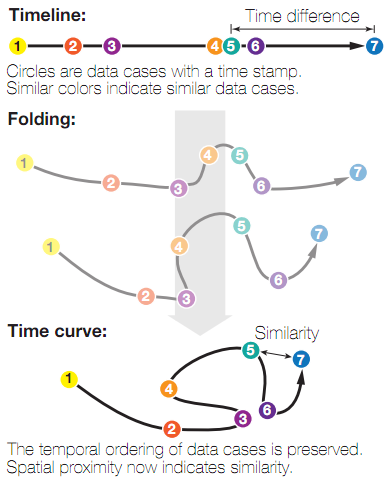
\includegraphics[width=\columnwidth]{images/time_curve_example.png}
    \caption{Three common correlation coefficient algorithms are compared on a sample data set. Note the consistency in visualization for the strong positive correlation between items 1 and 6, and the strong negative correlation between items 4 and 5.}
    \label{fig:time_curve_example}
\end{figure}


\subsection{}

\subsection{}

\subsection{}

\subsection{}



\section{Multidimensional Scaling for Characterizing Correlation Families}

\subsection{}

\subsection{}

\subsection{}

\subsection{}